%==============================================================================
%  PRL-style course report  —  EMPTY TEMPLATE / SCAFFOLD
%
%  Compile (run TWICE, plus bibtex, to resolve refs and citations):
%      pdflatex main
%      bibtex   main
%      pdflatex main
%      pdflatex main
%==============================================================================

% --- Document class -----------------------------------------------------------
% aps      : American Physical Society house style
% prl      : Physical Review Letters layout (two-column, PRL margins/fonts)
% reprint  : journal-like two-column output (use 'preprint' for a 1-col draft)
% amsmath/amssymb : math
% superscriptaddress : compact author/affiliation formatting
\documentclass[
  aps,
  prl,
  reprint,
  amsmath,
  amssymb,
  superscriptaddress,
  floatfix
]{revtex4-2}

% --- Packages -----------------------------------------------------------------
\usepackage{graphicx}   % figures
\usepackage{float}      % [H] = pin a figure in place (same column, no float)
\usepackage{tikz}       % lattice schematic (Kitaev honeycomb)
\usetikzlibrary{calc}   % (P)!t!(Q): point a fraction t along an edge
\usetikzlibrary{arrows.meta} % Stealth arrow tips
\usepackage{bm}         % bold math symbols (\bm)
\usepackage{braket}     % \ket{}, \bra{}, \braket{} (handy for spins)
\usepackage{physics}    % optional: \dd, \pdv, etc. (remove if it clashes)
\usepackage{xcolor}     % colored TODO notes; remove before final
\usepackage[colorlinks=true,allcolors=blue]{hyperref}
\usepackage{subcaption} % (a)/(b) subpanels within one figure

% Path to figures (PDFs). Adjust if you keep plots elsewhere.
\graphicspath{{figures/}{../Note/Plots/}{../Plots/}}

% A visible placeholder marker. Delete \todo lines as you write.
\newcommand{\todo}[1]{\textcolor{red}{[\textbf{TODO:} #1]}}
\newcommand{\numberthis}{\refstepcounter{equation}\tag{\theequation}}
\renewcommand{\norm}[1]{\left\lVert #1 \right\rVert}
\newcommand{\bfvec}[1]{\mathbf{#1}}
\renewcommand{\H}{\mathcal{H}}
\newcommand{\oL}{\hat{L}}
\newcommand{\oK}{\hat{K}}
\newcommand{\kpi}{\ket{\psi_{\pi}}}
\newcommand{\bpi}{\bra{\psi_{\pi}}}
\newcommand{\df}{\frac{\dd}{\dd x}}
\newcommand{\omP}{\hat{\mathcal{P}}}
\newcommand{\ee}{\mathrm{e}}
\newcommand{\pp}{\partial}
\newcommand{\oThe}{\hat{\Theta}}
\newcommand{\oS}{\hat{S}}
\newcommand{\ccM}{\mathcal{M}}
\renewcommand{\pdv}[2]{\frac{\pp #1}{\pp #2}}
\renewcommand{\dd}{\mathrm{d}}
\renewcommand{\O}{\mathcal{O}}
\newcommand{\he}{\hat{\ee}}
\newcommand{\oPi}{\hat{\Pi}}
\newcommand{\rhs}{R.H.S }
\newcommand{\lhs}{L.H.S }
\newcommand{\ii}{\mathrm{i}}
\newcommand{\ox}{\hat{x}}
\newcommand{\R}{\mathbb{R}}
\renewcommand{\op}{\hat{p}}
\renewcommand{\abs}[1]{\left| #1 \right|}
\renewcommand{\comm}[2]{\left[ #1 , #2 \right]}
\newcommand{\anticomm}[2]{\left\{ #1 , #2 \right\}}
\newcommand{\C}{\mathcal{C}}
\newcommand{\ra}{\rightarrow}
\newcommand{\Ra}{\Rightarrow}
\newcommand{\oO}{\hat{O}}
\newcommand{\I}{\mathbb{I}}
\newcommand{\avg}[1]{\langle #1 \rangle}
\usepackage[capitalise]{cleveref}
\newcommand{\FA}{F(\hat{A})}
\newcommand{\FB}{F(\hat{B})}
\renewcommand{\Tr}[1]{\mathrm{Tr}\left( #1 \right) }
\newcommand{\oA}{\hat{A}}
\newcommand{\oB}{\hat{B}}
\newcommand{\orho}{\hat{\rho}}
\newcommand{\U}{\hat{U}}
\newcommand{\ro}[1]{\hat{\mathcal{#1}}}
\newcommand{\kps}{\ket{\psi}}
\newcommand{\kph}{\ket{\phi}}
\newcommand{\bps}{\bra{\psi}}
\newcommand{\bph}{\bra{\phi}}
\newcommand{\mean}[1]{\left\langle #1 \right\rangle}
\newcommand{\basispsi}{\{\ket{\psi_i}\}}
\newcommand{\oH}{\hat{H}}
\newcommand{\wfr}{\Psi(\vec{r},t)}
\newcommand{\oI}{\hat{\mathbb{I}}}
\newcommand{\wf}{\Psi(x,t)}
\newcommand{\upket}{\ket{\uparrow}}
\newcommand{\downket}{\ket{\downarrow}}
\newcommand{\upbra}{\bra{\uparrow}}
\renewcommand{\a}{\hat{a}}
\newcommand{\adag}{\hat{a}^ \dag}
\newcommand{\oX}{\widehat{X}}
\newcommand{\oP}{\widehat{P}}
\newcommand{\oN}{\widehat{N}}
\newcommand{\downbra}{\bra{\downarrow}}
\newcommand{\ketshoizero}{\ket{\psi_ \nu}}
\newcommand{\brashoizero}{\bra{\psi_ \nu}}
\newcommand{\ketsho}{\ket{\psi_ \nu^i}}
\newcommand{\brasho}{\bra{\psi_ \nu^i}}
\newcommand{\kn}{\ket{n}}
\newcommand{\bn}{\bra{n}}
\newcommand{\oU}{\hat{U}}
\newcommand{\oT}{\hat{T}}
\renewcommand{\thefootnote}{\arabic{footnote}}
\newcommand{\ddx}[1]{\frac{\dd}{\dd #1}}
\newcommand{\oG}{\hat G}
\newcommand{\Z}{\mathbb{Z}}
\newcommand{\oR}{\hat{R}}
\newcommand{\boL}{\hat{\bfvec{L}}}
\newcommand{\Ylm}{Y_l^m}
\newcommand{\ylm}[2]{Y_{#1}^{#2}}
\newcommand{\ddxx}[2]{\frac{\dd^2 #1}{\dd #2 ^2}}
\newcommand{\spc}[1]{\bar{#1}}
\newcommand{\opi}{\hat{\pi}}
\newcommand{\bs}[1]{\boldsymbol{#1}}
\newcommand{\oJ}{\hat{J}}
\newcommand{\Ei}[1]{E^{(#1)}}
\newcommand{\oV}{\hat{V}}
\renewcommand{\oc}{\hat{c}}
\newcommand{\of}{\hat{f}}
\newcommand{\oga}{\hat \gamma}
\newcommand{\obx}{\hat b^x}
\newcommand{\oby}{\hat b^y}
\newcommand{\obz}{\hat b^z}
\newcommand{\osx}{\sigma^x}
\newcommand{\osy}{\sigma^y}
\newcommand{\osz}{\sigma^z}
%==============================================================================
\begin{document}

% --- Title and authors --------------------------------------------------------
\title{Kitaev Honeycomb model}

\author{Zhenming Shi}
\affiliation{Leipzig University}

\date{\today}

% --- Abstract -----------------------------------------------------------------
% PRL abstract: one paragraph, no citations, ~5 sentences. Write it LAST.
\begin{abstract}
The Kitaev honeycomb model is one exactly solvable 2 dimensional interacting spin model which is rare in 2 dimensional systems.
It has direction dependent bond strengths with spin interactions. The key point to exactly solving it is the conserved plaquette vortices and static $\mathbb{Z}_2$ gauge field obtained by four Majorana representation. The Hamiltonian is read as a quadratic form by such point to be exactly solvable. 
The ground state is realized by Lieb's theorem on vortex-free sector, the phase diagrams contains three gapped phases and one gapless phase with two Dirac cones. A weak magnetic field is applied by third order of perturbation to open the gap and make it topological. It is then realized as a three-spin term. 
By four Majorana representation, it becomes a next nearest neighbour Majorana hopping which breaks time reversal symmetry, opens the gap and yields non-zero Chern number.
\end{abstract}

\maketitle

% Ragged bottom: don't vertically stretch sparse columns to fill the page.
% While the draft is short, flush-bottom (REVTeX default) opens big gaps around
% equations and floats. Remove this line once the columns are full for standard
% PRL flush-bottom justification.
\raggedbottom

% Number sections so that \cref/\ref to \label{sec:...} resolve (PRL suppresses
% section numbers by default, which leaves section cross-references blank).
\setcounter{secnumdepth}{3}

%==============================================================================
\section{Introduction}
\label{sec:intro}
In two dimension, it is rare to find exactly solvable models. The Kitaev honeycomb model \cite{Kitaev2006} is one exactly solvable model, initially as a platform for non-Abelian anyons with rich physics much beyond the original goal: its ground state is a $\mathbb{Z}_2$ quantum spin liquid, its excitations are Majorana fermions and static $\mathbb{Z}_2$ gauge fluxes. In a magnetic field a chiral topological phase is realized on the gapped phase.
% optional: \cite{JackeliKhaliullin2009, Trebst2022} for Kitaev materials

The key to exact solving it is the conserved $\mathbb{Z}_2$ plaquette fluxes: written in terms of four Majorana operators per spin, they become a static gauge field and the model reduces to a graphene-like free-fermion problem. 
After presenting the solution (\cref{sec:model,sec:method,sec:results}), we compute the phase diagram, the Chern number $\mathcal{C}=\pm1$ (similar with the Haldane model \cite{Haldane1988} but different type of particles). 
All details about calculation and further explanations can be found in Supplemental Material \cite{SM}.
% --- Kitaev honeycomb lattice schematic --------------------------------------
% Three-bond coloring: z = vertical link, x = up-right (/) link, y = up-left
% (\) link. Each B-site of the triangular sublattice emits its three distinct
% links, so every bond is drawn exactly once (boundary links are left dangling,
% as in the standard figure).


%==============================================================================
\section{The Model}
\label{sec:model}
% Suggested role: define the model / Hamiltonian and your conventions.
The Hamiltonian of the model is(\cref{fig:lattice}) \cite{Kitaev2006}:
\begin{align}
  \hat H = - J_x \sum_{\mean{j,k}_x} \osx_j \osx_k - J_y \sum_{\mean{j,k}_y} \osy_j \osy_k - J_z \sum_{\mean{j,k}_z} \osz_j \osz_k
\end{align}

% --- Kitaev honeycomb lattice: small 3-hexagon cluster (2 top, 1 bottom) ------
% Pointy-top hexagons, circumradius 1 (edge length 1).
% Centres: B=(0,0); TL=(-s,1.5); TR=(s,1.5)   with s = sqrt(3)/2.
% Coloring:  "/" edges = x,  "\" edges = y,  vertical edges = z.
% Sublattice nodes: filled at {T,LR,LL}, open at {UR,Bo,UL} (consistent split).
% No \resizebox -> a fixed `scale` keeps the cluster small; bump `scale` to
% enlarge, or move the three centres to rearrange the cluster.
% --- Fig. 1: (a) plaquette + bond types, (b) four-Majorana decomposition -----
% (a) is Note/Plots/invariant.pdf: one plaquette p, sites numbered 1..6
% (filled/open = odd/even sublattice), bonds labelled x,y,z as in W_p.
% (b) resolves each site into a matter Majorana gamma (black) + gauge
% b^x,b^y,b^z (colored), with each alpha-bond's two like-colored b's paired
% into u_{jk} = i b^a_j b^a_k.
\begin{figure}[t]
  \centering
  % ===== (a) plaquette with bond types =====
  \begin{subfigure}[b]{0.49\columnwidth}
    \centering
    \includegraphics[width=0.8\linewidth]{invariant}
    \caption{}
    \label{fig:lattice}
  \end{subfigure}\hfill
  % ===== (b) four-Majorana (parton) decomposition =====
  \begin{subfigure}[b]{0.49\columnwidth}
    \centering
    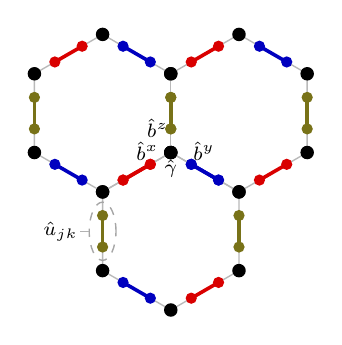
\begin{tikzpicture}[scale=1, line width=0.6pt,
        gam/.style={fill=black,draw=black},
        bl/.style={font=\scriptsize\itshape,inner sep=1pt}]
      \pgfmathsetmacro{\s}{sqrt(3)/2}
      \def\bt{0.30}   % fraction along each edge where the gauge Majorana b sits
      \def\gr{0.075}  % gamma (matter) dot radius
      \def\br{0.060}  % b (gauge) dot radius
      \colorlet{cx}{red!85!black}
      \colorlet{cy}{blue!75!black}
      \colorlet{cz}{olive!80!black}
      \newcommand{\edgemaj}[3]{%
        \draw[gray!55,line width=0.5pt] (#1) -- ($(#1)!\bt!(#2)$);
        \draw[gray!55,line width=0.5pt] (#2) -- ($(#2)!\bt!(#1)$);
        \draw[#3,line width=1.3pt]      ($(#1)!\bt!(#2)$) -- ($(#2)!\bt!(#1)$);
        \filldraw[#3] ($(#1)!\bt!(#2)$) circle(\br);
        \filldraw[#3] ($(#2)!\bt!(#1)$) circle(\br);
      }
      \newcommand{\hexmaj}[2]{%
        \coordinate (T)  at (#1,{#2+1});
        \coordinate (UR) at ({#1+\s},{#2+0.5});
        \coordinate (LR) at ({#1+\s},{#2-0.5});
        \coordinate (Bo) at (#1,{#2-1});
        \coordinate (LL) at ({#1-\s},{#2-0.5});
        \coordinate (UL) at ({#1-\s},{#2+0.5});
        \edgemaj{UL}{T}{cx}\edgemaj{T}{UR}{cy}\edgemaj{UR}{LR}{cz}%
        \edgemaj{LR}{Bo}{cx}\edgemaj{Bo}{LL}{cy}\edgemaj{LL}{UL}{cz}%
        \foreach \v in {T,UR,LR,Bo,LL,UL}{\filldraw[gam] (\v) circle(\gr);}
      }
      \hexmaj{0}{0}\hexmaj{-\s}{1.5}\hexmaj{\s}{1.5}
      % label the fully-coordinated central site at (0,1)
      \node[bl] at (-0.3,1.02) {$\obx$};
      \node[bl] at ( 0.42,1.02) {$\oby$};
      \node[bl] at (-0.17,1.31) {$\obz$};
      \node[bl] at ( 0.00,0.8) {$\oga$};
      % highlight one link variable u_{jk} on the bottom-left z-bond
      \draw[gray!70,dashed,line width=0.5pt] (-\s,0) ellipse [x radius=0.17, y radius=0.37];
      \draw[gray!60,line width=0.4pt] (-1.15,0) -- ({-\s-0.17},0);
      \node[bl] at (-1.40,0) {$\hat u_{jk}$};
    \end{tikzpicture}
    \caption{}
    \label{fig:majorana}
  \end{subfigure}
  \caption{(a)~A plaquette $p$: The bond strengths depend on $x,y,z$ directions, filled site is 
    sublattice, blank site is even sublattice; the site numbering $1,\dots,6$ and the
    outgoing bond labels are those entering the flux operator $\hat W_p$
    of \cref{eq:Wp}.
    (b)~Four-Majorana representation: each spin becomes four Majoranas
    $\oga, \obx,\oby,\obz$ ($x$ red,
    $y$ blue, $z$ olive); on every $\alpha$-bond the Majorana bond operator:
    $\hat u_{jk}=\ii\,\hat b^{\alpha}_j\hat b^{\alpha}_k$.}
  \label{fig:honeycomb}
\end{figure}

with bond-direction dependent interaction coefficients $J_x,J_y,J_z$.
The operator $\hat K_{jk} = \sigma^{\alpha}_j \sigma^{\alpha}_k$, $\alpha \in \{x,y,z\}$ is defined as bond operator, with $\alpha$ determined by the direction of the bond. The plaquette operator is defined as: 
\begin{equation}
  \hat{W}_p = \sigma_1^x \sigma_2^y \sigma_3^z
              \sigma_4^x \sigma_5^y \sigma_6^z
            = \oK_{12}\oK_{23}\oK_{34}\oK_{45}\oK_{56}\oK_{61}.
  \label{eq:Wp}
\end{equation}
$p$ is the label of the plaquette. The $\hat W_p$ commute with one another and
with every bond operator $\oK_{jk}$ (any two overlapping operators share an
even number of anticommuting Pauli matrices), hence $[\hat{W}_p, \oH] = 0$, i.e., 
the $\hat{W}_p$ are conserved, and since $\hat W_p^2 = \oI$ the Hilbert
space splits into sectors labelled by $w_p = \pm 1$ on every plaquette.
Each plaquette has six vertices and each vertex is shared by three
plaquettes, so $n$ vertices give $n/2$ plaquettes: the $2^n$-dimensional
Hilbert space splits into $2^{n/2}$ flux sectors of dimension $2^{n/2}$
each. This still can not fix the problem, the so-called parton construction gives the key to exact solution.

%==============================================================================
\section{Representing Spins by Majorana Operators}
\label{sec:method}
Kitaev represents each spin by four Majorana operators
$\obx,\oby,\obz,\oga$, shown in \cref{fig:majorana}. Majorana operators as a decomposition of complex fermionic operator: $\hat f = \oc + \oc^ \dag,\; \hat f^ \dag = (\oc -\oc^ \dag)/\ii$. 
This enlarges the dimension of space on each site: $2$ dimensional Fock space of one spin to $4$ dimensional Fock space of four Majoranas.
Pauli operators becomes $\tilde{\sigma}^ \alpha = \ii \hat b^ \alpha \oga$ and The bond operators become $\hat{K}_{jk} = - \ii \hat{u}_{jk} \oga_j \oga_k$ with $\hat{u}_{jk}:= \ii \hat{b}^\alpha_j\hat{b}^\alpha_k$ which is Hermitian and squares to one. To fix the dimension enlarged problem, operator $\hat{D}:= \obx \oby \obz \oga$ is used to determine the physical subspace: a state $\ket{\xi}$ is physical iff $\hat D \ket{\xi} = \ket{\xi}$. One can find $\comm{\hat D}{\oH} = 0$, which leaves physical subspace invariant. 




%==============================================================================
\section{Spectrum and phase diagram}
\label{sec:results}
With the Majorana bond operators $\hat{u}_{jk}= \ii \hat{b}^ \alpha_j \hat{b}^ \alpha_k$ defined above, the Hamiltonian becomes a quadratic form of free Majorana fermions,
$\tilde{H} = \frac{\ii}{4}\sum_{j,k} \oA_{jk} \oga_j \oga_k$, with
$\oA_{jk} = 2 J_{\alpha_{jk}} \hat u_{jk}$ on connected sites and zero
otherwise.
$\hat{u}_{jk}$ commutes with $\tilde{H}$ and has eigenvalues $\pm 1$, forms a static $\mathbb{Z}_2$ gauge field. Once a configuration $\{u_{jk}\}$ is fixed, $\tilde{H}$ can be exactly diagonalized; from its ground state $\ket{\tilde{\Psi}_u}$ the physical state is recovered by the projection $\ket{\Psi_w} = [\prod_j (1+\hat{D_j})/2] \ket{\tilde{\Psi}_u}$.
The label $w$ is the gauge-equivalence class of $\{u_{jk}\}$, which is characterized by the fluxes $w_p = \prod_{(j,k)\in \pp p} u_{jk} = \pm 1$ ($j$ odd, $k$ even). There are many possible configurations of $\{u_{jk}\}$,
by Lieb's theorem \cite{Lieb1994} the ground state lies in the flux-free sector with $w_p = +1$ on every plaquette, and we can choose the simplest gauge, $u_{jk}=+1$ on all links.

The Bravais lattice of honeycomb lattice is not the honeycomb itself, but half of the lattice. We place the odd ($A$) sublattice at the cell origin $\bm R$ and
reach the even ($B$) sublattice by the bond vectors $\bm\delta_\alpha$
($A\to B$), with $\bm n_1=\bm\delta_z-\bm\delta_y$ and $\bm
n_2=\bm\delta_z-\bm\delta_x$; explicit conventions and geometry are given in the SM
\cite{SM}, Fig.~S1. The real-space Hamiltonian in the ${u_{jk}=1}$ gauge is
\begin{align}
  \tilde{H}_u = \ii \sum_{\bm R,\alpha} J_\alpha\, \oga_{\bm R}^A\, \oga_{\bm R+\bm\delta_\alpha}^B .
\end{align}
Applying fourier transformation in the periodic gauge
and choosing the sublattice spinor
$\chi_{\bm q}=(\tilde\gamma^A_{\bm q},\,\tilde\gamma^B_{\bm q})^{\mathsf T}$,
the Hamiltonian in Bloch form is
\begin{align}
  \tilde{H}_u = \frac{1}{2} \sum_{\bm q} \chi_{\bm q}^\dag h(\bm q) \chi_{\bm q}, \quad h(\bm q) = \begin{pmatrix}
    0 & \ii f(\bm q) \\
    - \ii f(\bm q)^* & 0
  \end{pmatrix}, \label{eq:bloch_Hamiltonian}
\end{align}
with factor
$f(\bm q)=\sum_\alpha J_\alpha \ee^{\ii \bm q\cdot\bm\delta_\alpha}$.
Expanding in Pauli matrices, $h(\bm q)=\bm d(\bm q)\cdot\bm\sigma$ gives $d_x = -\Im f$, $d_y = -\Re f$, and $d_z = 0$.
The vanishing of $d_z$ reflects the chiral (sublattice) symmetry: $\bm d$ stays in the $xy$-plane over the whole Brillouin zone. The bulk dispersion is
\begin{align}
  \epsilon_\pm(\bm q) = \pm \abs{f(\bm q)} = \pm\sqrt{d_x^2+d_y^2}.
\end{align}

The gap closes at $f(\bm q) = 0$. Geometrically, each term $J_{\alpha} \ee^{\ii \bm q \cdot \bm \delta_ \alpha}$ is a vector of length $\abs{J_{\alpha}}$ in the complex plane; their sum vanishes only if the three vectors close into a triangle, which requires the triangle inequalities $\abs{J_x} \leq \abs{J_y} + \abs{J_z}$ (and cyclic).
When the inequalities hold strictly the spectrum is gapless (phase B); when
one is violated, it is gapped (phase $A_\alpha$); see
\cref{fig:phase_diagram_ground}.

\begin{figure}[t]
  \centering
  \includegraphics[scale=0.38]{HC_1_phase_diagram.pdf}
  \caption{Phase diagram by constraint $J_x+J_y+J_z=1$: the central
triangle is the gapless phase B, bounded by $J_\alpha=\tfrac12$;
the corners three are the gapped phases $A_x,A_y,A_z$. Shading: bulk gap
$\Delta$. In phase B it is clearly gapless.}
  \label{fig:phase_diagram_ground}
\end{figure}

At the symmetric point $J_x=J_y=J_z$, the three bonds become equivalent and
the Hamiltonian acquires a $C_3$ rotational symmetry. Since the corners of the
Brillouin zone are the fixed points of $C_3$, the solutions of $f(\bm q)=0$ are
pinned there: the two Dirac points locate exactly at the inequivalent conical points 
$\pm\bm K$, and linearizing $f(\bm q)$ about them yields a graphene-like
linear dispersion (SM \cite{SM}, Fig.~S2).

Chiral symmetry constrain $d_z(\bm q)$ strictly to be zero, so gap closing only requires
$d_x=d_y=0$: two conditions on two dimensional Brillouin zone, generically
satisfied at the Dirac points. A nonzero $d_z$ adds a
third condition, which is impossible to find the solution, so breaking the chiral symmetry
gaps the Dirac points and phase B becomes gapped.

\section{Time-reversal breaking and the Chern number}
The time reversal operator acts on the Hamiltonian \cref{eq:bloch_Hamiltonian} as $\hat T = \sigma_z \mathcal{K}$, the detail could be find in SM \cite{SM}. The result: $\sigma_z h^*(\bm q)\sigma_z = h(-\bm
q)$, and matching Pauli matrices gives
\begin{align}
  d_x(-\bm q) = -d_x(\bm q), \quad d_y(-\bm q) = d_y(\bm q), \quad 
  d_z(-\bm q) = +d_z(\bm q).
\end{align}
Thus time-reversal symmetry forces $d_z(\bm q)$ to be even: a
time-reversal-symmetric mass gives the two Dirac points {equal} masses
and the Chern number vanishes (shown below); a topological gap needs an
odd mass, the time-reversal breaking mass, which requires broken time-reversal symmetry.


A weak external magnetic field $\bm h = (h_x, h_y, h_z)$ breaks time-reversal
symmetry and enters as the perturbation $V = -\sum_j \bm h \cdot
\bm\sigma_j$; for simplicity, we work at the isotropic point $J_x = J_y = J_z \equiv J$.
Since $\sigma_j^\alpha = \ii\, \hat b_j^\alpha \gamma_j$ carries a single
gauge Majorana, which anticommutes with the link operator $\hat u_{jk}$ on
the $\alpha$-bond at site $j$, meaning $\hat u_{jk}$ is flipped by $\sigma$;
the bond is shared by two plaquettes, so both $w_p$ flip from $+1$ to $-1$
and the state leaves the vortex-free sector.

To obtain the effective Hamiltonian within the vortex-free sector we use the 
Schrieffer--Wolff (perturbative) expansion in $V$,
\begin{align}
  H_{\text{eff}} = \sum_{n=1}^{\infty} H^{(n)}_{\text{eff}},
  \qquad
  H^{(n)}_{\text{eff}} = \Pi_0 V \left( G_0'\, V \right)^{n-1} \Pi_0 ,
\end{align}
where $\Pi_0=\prod_p \tfrac{1+\hat W_p}{2}\,\prod_j \tfrac{1+\hat D_j}{2}$
projects onto the vortex-free sector and $G_0'$ is the unperturbed Green's
function with that sector removed; since the intermediate two-vortex states
cost an energy of order $\abs{J}$, $G_0'(E_0) \simeq -(1-\Pi_0)/\abs{J}$.
Each factor of $V$ breaks time reversal symmetry, so the
$n$-th order term picks up $(-1)^n$ under $\hat T$: only odd orders can
generate the time-reversal breaking mass $d_z$.

At first order, $H^{(1)}_{\text{eff}} = \Pi_0 V \Pi_0 = 0$: a single
$\sigma_j^\alpha$ flips $w_p$ on the two plaquettes adjacent to its bond and
takes the state out of the vortex-free sector, so the left first $\Pi_0$ projects
it to zero. At second order, $H^{(2)}_{\text{eff}}=\Pi_0 V G_0' V
\Pi_0\neq0$, since the second perturbation term can annihilate the vortex pair
created by the first. However, with $n=2$ factors of $\bm h$ it is still
time-reversal symmetric and can not make the gap topological, so we drop it. The leading time-reversal breaking
term is the third order, $H^{(3)}_{\text{eff}}=\Pi_0 V G_0' V G_0' V
\Pi_0$. The only possible configuration is three spin interactions at nearest three bonds, or 3 bond near the same site (SM \cite{SM}, Fig.~S3). With two Green's functions $G_0'\sim
-1/\abs{J}$ and three powers of $\bm h$ it takes the form
\begin{align}
  H^{(3)}_{\text{eff}} \sim -\kappa \sum_{\langle jkl\rangle}
  \sigma_j^x\, \sigma_k^y\, \sigma_l^z,
  \qquad
  \kappa \sim \frac{h^x h^y h^z}{\abs{J}^2},
  \label{eq:H3_spin}
\end{align}
where in each triple the central spin $\sigma_l^z$ sits on an even ($B$) site
$l$, and $\sigma_j^x, \sigma_k^y$ sit on the two odd ($A$) sites linked to $l$
by the $x$- and $y$-bonds.

Inserting the Majorana spin expression $\sigma_j^ \alpha$ and $\hat D = 1$ into third order term, with a fixed gauge $\{u=1\}$, gives a next-nearest neighbour hopping between same-sublattice sites,
$\sigma_j^x \sigma_k^y \sigma_l^z = -\ii\,
\oga_j \oga_k$ with $j,k$ displaced by $\bm n_1-\bm n_2$ (geometry in the
\cite{SM}, Fig.~S4) which is identical to the structure of the Haldane model
\cite{Haldane1988}.
We sum over the lattice. An $A$-centred process carries the opposite sign
on the $B$ sublattice, since the directed bond reverses. So the
same-sublattice hopping contributes the diagonal term $d_z(\bm q)\,\sigma_z$
to the Bloch Hamiltonian. Fourier transforming (\cite{SM}) gives
\begin{align}
  d_z(\bm q) = 6\kappa\Big[\sin(\bm q\cdot\bm n_1) + \sin(\bm q\cdot\bm n_2)
  + \sin\!\big(\bm q\cdot(\bm n_1-\bm n_2)\big)\Big],
  \label{eq:dz}
\end{align}
As a sum of sines, $d_z$ is odd,
$d_z(-\bm q)=-d_z(\bm q)$: the field breaks time-reversal symmetry,
and the Bloch Hamiltonian becomes 
\begin{align}
  h(\bm q) = \begin{pmatrix} d_z(\bm q) & \ii f(\bm q) \\ 
  -\ii f^*(\bm q) & -d_z(\bm q)\end{pmatrix} = \bm d(\bm q)\cdot\bm\sigma,
  \label{eq:h_gapped}
\end{align}

% ========== gapped spectrum ==========
\paragraph{Gapped spectrum.}
For $h=\bm d\cdot\bm\sigma$ the eigenvalues are $\pm\abs{\bm d}$. Since 
$d_x^2+d_y^2=\abs{f(\bm q)}^2$ as previous solution, the dispersion is
\begin{align}
  \varepsilon_\pm(\bm q) = \pm\sqrt{\abs{f(\bm q)}^2 + d_z(\bm q)^2}.
  \label{eq:gapped_spectrum}
\end{align}
As the solution given in gapless phase B, $\abs{f(\bm q)}^2$ still vanishes at the two Dirac points $\pm \bm K$. With non-zero mass term the gap at the Dirac points separates as:
\begin{align}
  d_z(\pm\bm K) = \mp 3\sqrt3\,\kappa,
  \quad
  \Delta = 2\abs{d_z(\bm K)} = 6\sqrt3\,\abs{\kappa}
  \label{eq:gap_value}
\end{align}
and the time-reversal breaking mass term will also make the gap topological.

\paragraph{Chern number.}
The topological invariant of a gapped two-dimensional system of noninteracting fermions is the Chern number of the occupied band \cite{TKNN1982},
\begin{align}
  \mathcal C = \frac{1}{2\pi}\int_{\text{BZ}}\Omega(\bm q)\,\dd^2q,
  \label{eq:chern_def}
\end{align}
where $\Omega(\bm q)$ is the Berry curvature of the negative-energy band. The integral reduces
to a sum of local contributions \cite{SM},
\begin{align}
  \mathcal C = \frac12\sum_{i=\pm\bm K}\operatorname{sgn}(m_i)\,\nu_i,
  \label{eq:chern_dirac}
\end{align}
where $\mathrm{sgn}(m_{\pm \bm K})= \mp \mathrm{sgn}(\kappa)$ is the mass and $\nu_i=\pm1$ the winding number at
each Dirac point. Linearizing $f$ gives $\nu_{\pm\bm K}=\mp1$: the two
windings are opposite, since the total winding over the
Brillouin-zone torus must vanish
\cite{NielsenNinomiya1981}. The masses are opposite as well,
$\operatorname{sgn}(m_{\pm\bm K})=\mp\operatorname{sgn}(\kappa)$. Hence
$\mathcal C = \operatorname{sgn}(\kappa)=\pm1$. 

%==============================================================================
\section{Conclusion}
\label{sec:conclusion}
The conserved plaquette vortices split the Hilbert space into flux sectors.
Together with the four Majorana representation, the model becomes free Majorana fermions in a static $\mathbb{Z}_2$ gauge field.
A triangular phase diagram is realized and contains one gapless phase similar to graphene with two Dirac points.
A weak magnetic field breaks the chiral and time reversal symmetry. At third order in perturbation theory it generates a next nearest neighbour hopping which gaps the two Dirac cones. The gapped phase carries a topological invariant, the Chern number $\mathcal{C}=\pm 1$.

% --- Acknowledgments (optional) -----------------------------------------------
\begin{acknowledgments}
  \emph{AI usage: Claude (Anthropic) was used as an assistant in this project.
For the figures, it provided coding help; the choice of what to plot and the
approach are my own. It also helped with the \LaTeX{} template and the formatting
of the report and supplementary material. The physics, derivations, and text are my own.}
\end{acknowledgments}

% --- Bibliography -------------------------------------------------------------
% Entries live in references.bib. apsrev4-2 is the PRL bibliography style.
\bibliographystyle{apsrev4-2}
\bibliography{references}

\end{document}